\documentclass[10pt,a4paper,twocolumn]{article}

% Idioma e codificação
\usepackage[utf8]{inputenc}
\usepackage[T1]{fontenc}
\usepackage[brazil]{babel}

% Layout de artigo
\usepackage[a4paper,top=2.2cm,bottom=2.2cm,left=1.8cm,right=1.8cm,columnsep=0.65cm]{geometry}
\usepackage{times}
\usepackage{microtype}
\usepackage{indentfirst}
\usepackage{setspace}
\setstretch{1.0}

% Matemática, figuras e tabelas
\usepackage{amsmath,amssymb}
\usepackage{graphicx}
\usepackage{booktabs}
\usepackage{tabularx}
\usepackage{array}
\usepackage{multirow}
\usepackage{caption}
\usepackage{subcaption}
\usepackage{float}
\usepackage{xcolor}
\usepackage{enumitem}
\usepackage[hidelinks]{hyperref}
\usepackage{cite}

% Diagramas
\usepackage{tikz}
\usetikzlibrary{shapes.geometric, arrows.meta, positioning}

% Listas compactas
\setlist[itemize]{noitemsep,topsep=2pt,leftmargin=*}
\setlist[enumerate]{noitemsep,topsep=2pt,leftmargin=*}

% Legendas compactas
\captionsetup{font=small,labelfont=bf}

\title{\textbf{Detecção de Formigueiros em Ortofotos Aéreas por Segmentação Semântica com U-Net}}

\author{
Isabelle Oliveira Bicudo\textsuperscript{1},
Rodolpho Ale\textsuperscript{1}\\[0.4cm]
\small Orientador: Prof. Dr. Wesley Nunes Gonçalves\\[0.2cm]
\textsuperscript{1}\small Faculdade de Computação Universidade Federal de Mato Grosso do Sul (UFMS)\\
\small Campo Grande MS Brasil
}

\date{}
\date{}

\begin{document}

\maketitle

\begin{abstract}
Este trabalho apresenta uma abordagem de segmentação semântica para detecção automática de formigueiros em ortofotos aéreas de talhões agrícolas. O problema é desafiador devido ao forte desbalanceamento entre fundo e classe de interesse, à baixa frequência de exemplos positivos e à semelhança visual entre formigueiros e regiões de solo exposto. A solução proposta utiliza uma arquitetura U-Net para segmentação binária, com pré-processamento das máscaras, normalização das imagens, transformações sincronizadas entre imagem e rótulo, augmentação da classe de interesse e pós-processamento por limiar de confiança e filtragem de regiões. Foram avaliadas diferentes configurações de treinamento e validação, considerando métricas de detecção e segmentação, como Precision, Recall, F1-Score, Dice e IoU. Os resultados indicam que a preparação dos dados e o tratamento do desbalanceamento, em conjunto com a estabilização da arquitetura (normalização e upsampling aprendido), foram determinantes para a evolução do modelo. A melhor configuração priorizou a detecção de formigueiros, alcançando Recall de 91,7\%, F1-Score de 83,1\% e IoU da classe formigueiro de 33,8\%. A análise dos erros mostrou que falsos positivos estão associados principalmente a solo avermelhado e marcas no terreno, enquanto falsos negativos ocorrem em formigueiros pequenos ou visualmente semelhantes ao fundo.
\end{abstract}

\noindent\textbf{Palavras-chave:} segmentação semântica; U-Net; formigueiros; ortofotos aéreas; visão computacional agrícola; desbalanceamento de classes.

\section{Introdução}

O monitoramento de pragas em lavouras é uma atividade essencial para reduzir perdas produtivas e orientar ações de manejo. Entre os problemas recorrentes em áreas agrícolas, a presença de formigueiros pode comprometer o desenvolvimento da cultura e exigir intervenções localizadas \cite{dellalucia2014}. Em grandes talhões, a inspeção manual demanda tempo, custo operacional e depende da experiência dos avaliadores em campo.

O uso de veículos aéreos não tripulados e ortofotos de alta resolução permite observar grandes extensões agrícolas com maior frequência \cite{tsouros2019}. Entretanto, a análise manual dessas imagens continua sendo trabalhosa, especialmente quando o alvo possui baixa representatividade espacial. Nesse contexto, técnicas de visão computacional e aprendizado profundo podem auxiliar na identificação automática de regiões de interesse \cite{kamilaris2018}.

Este trabalho aborda a detecção de formigueiros como um problema de segmentação semântica binária. Dado um recorte RGB de uma ortofoto aérea, o objetivo é classificar cada pixel como fundo ou formigueiro. A segmentação semântica é adequada ao problema porque os formigueiros possuem formato irregular, o que torna a representação por caixas delimitadoras menos precisa.

Os principais desafios encontrados foram: (i) predominância de pixels de fundo; (ii) pequena área ocupada pelos formigueiros, mesmo nas imagens positivas; e (iii) semelhança visual entre solo exposto e formigueiros. Para enfrentar esses fatores, foi desenvolvida uma pipeline baseada em U-Net, com pré-processamento das máscaras, normalização das imagens, transformações sincronizadas entre imagem e máscara, augmentação da classe minoritária e análise sistemática das métricas de validação.
A hipótese é que, em cenários de segmentação semântica com forte desbalanceamento e poucos exemplos positivos, estratégias sistemáticas de preparação de dados e de tratamento do desbalanceamento (padronização de máscaras, transformações sincronizadas, augmentação da classe minoritária, funções de custo especializadas e calibração de limiar) produzem ganhos substanciais e incrementais na detecção e na segmentação da classe minoritária.

As contribuições deste trabalho são:

\begin{itemize}
    \item avaliação sistemática do impacto da preparação de dados em segmentação semântica altamente desbalanceada;

    \item análise experimental do trade-off entre Recall e IoU em detecção de formigueiros;

    \item proposta de pipeline robusto para tratamento de máscaras RGB em segmentação agrícola;

    \item investigação do impacto combinado de Tversky Loss, Focal Loss e Lovász Loss em cenários de baixa representatividade da classe positiva;

    \item análise qualitativa dos principais padrões de erro do modelo.
\end{itemize}

\section{Trabalhos Relacionados}

A segmentação semântica com redes neurais convolucionais foi consolidada a partir das Fully Convolutional Networks (FCN) \cite{long2015}, que substituíram camadas densas por convoluções para gerar mapas densos de classificação. Posteriormente, a U-Net \cite{ronneberger2015} tornou-se uma das arquiteturas mais utilizadas em segmentação por combinar um caminho de contração, responsável por capturar contexto, com um caminho de expansão, responsável por recuperar resolução espacial. As conexões diretas entre encoder e decoder permitem preservar informações finas de localização, sendo úteis para objetos pequenos e irregulares.

Em tarefas agrícolas, redes profundas têm sido aplicadas a imagens de drones e satélites para identificação de plantas daninhas \cite{milioto2018,sa2018}, doenças \cite{mohanty2016}, falhas de plantio e degradação do solo \cite{kamilaris2018}. Estudos nessa área indicam que modelos convolucionais são adequados para padrões visuais locais, mas sofrem com variações de iluminação, escala e textura. Problemas de segmentação em imagens aéreas também costumam apresentar desbalanceamento severo, pois a classe de interesse ocupa pequena fração dos pixels \cite{sa2018}.

Para lidar com esse cenário, funções de custo baseadas em sobreposição, como Dice Loss \cite{milletari2016} e Tversky Loss \cite{salehi2017}, são utilizadas para reduzir o domínio da classe majoritária. A Focal Loss \cite{lin2017} também é empregada em problemas com grande quantidade de exemplos fáceis, pois reduz a contribuição de pixels classificados corretamente com alta confiança. Além disso, estratégias de augmentação \cite{buslaev2020} e seleção de patches \cite{ronneberger2015} são importantes para aumentar a exposição do modelo a regiões relevantes.

Especificamente para a detecção de formigueiros (ninhos de formigas cortadeiras), trabalhos recentes empregaram sensoriamento remoto: Santos et al.~\cite{santos2019} mapearam ninhos de \textit{Atta sexdens} em plantios de teca a partir de imagens de satélite, e dos Santos et al.~\cite{dossantos2022} detectaram e mediram ninhos com \textit{deep learning} sobre imagens de VANT.

Este trabalho diferencia-se por abordar a detecção de formigueiros como segmentação semântica pixel a pixel e por avaliar sistematicamente o impacto da preparação de dados e do tratamento do desbalanceamento no desempenho. Além disso, separa formalmente métricas de detecção e de segmentação, permitindo análise mais precisa do trade-off entre Recall e IoU em cenários de objetos pequenos e classes altamente desbalanceadas.

\section{Materiais e Métodos}

A Figura~\ref{fig:pipeline} resume a pipeline proposta. De forma resumida, o processamento ocorre nas seguintes etapas:

\begin{enumerate}
    \item \textbf{Leitura dos dados:} carrega-se o recorte RGB da ortofoto e a máscara correspondente, que marca onde estão os formigueiros.
    \item \textbf{Decodificação da máscara:} a máscara vem com regiões pintadas em cores; cada cor é convertida em um rótulo numérico (fundo, formigueiro ou área ignorada) que o modelo consegue interpretar.
    \item \textbf{Normalização e transformações sincronizadas:} os valores dos pixels são ajustados a uma escala comum e transformações geométricas (rotações e espelhamentos) são aplicadas de forma idêntica à imagem e à máscara, para que permaneçam alinhadas.
    \item \textbf{Predição pela U-Net:} a rede analisa o recorte e atribui a cada pixel uma probabilidade de pertencer a um formigueiro.
    \item \textbf{Pós-processamento:} um limiar de confiança decide quais pixels são considerados formigueiro e um filtro remove regiões muito pequenas ou improváveis, gerando a máscara final.
\end{enumerate}

\begin{figure*}[t]
\centering
\begin{tikzpicture}[
box/.style={rectangle, draw=black, rounded corners=3pt, minimum width=2.0cm, minimum height=0.8cm, align=center, font=\small},
arr/.style={-{Stealth[length=4pt]}, thick}
]
\node[box] (a) {Imagem RGB\\+ máscara};
\node[box, right=0.5cm of a] (b) {Decodificação\\RGB $\rightarrow$ classes};
\node[box, right=0.5cm of b] (c) {Normalização\\e filtros};
\node[box, right=0.5cm of c] (d) {Augmentação\\sincronizada};
\node[box, right=0.5cm of d] (e) {U-Net};
\node[box, right=0.5cm of e] (f) {Threshold\\+ regiões};
\node[box, right=0.5cm of f] (g) {Máscara\\predita};
\draw[arr] (a) -- (b);
\draw[arr] (b) -- (c);
\draw[arr] (c) -- (d);
\draw[arr] (d) -- (e);
\draw[arr] (e) -- (f);
\draw[arr] (f) -- (g);
\end{tikzpicture}
\caption{Visão geral da pipeline de segmentação semântica para detecção de formigueiros.}
\label{fig:pipeline}
\end{figure*}

\subsection{Dataset}

O dataset é composto por recortes de ortofotos aéreas RGB e suas respectivas máscaras de segmentação. As imagens utilizadas possuem dimensão padrão de $256 \times 256$ pixels. As máscaras foram produzidas manualmente e codificadas por cores, sendo necessário convertê-las para rótulos numéricos antes do treinamento.

A Tabela~\ref{tab:dataset} apresenta a distribuição das imagens utilizadas nos experimentos, indicando quantas contêm formigueiro (positivas) e quantas não contêm (negativas). Os valores referem-se ao número de imagens (recortes de $256\times256$ px), não a pixels.

\begin{table}[H]
\centering
\caption{Distribuição do dataset, em número de imagens ($256\times256$ px) por conjunto.}
\label{tab:dataset}
\begin{tabular}{lrrr}
\toprule
\textbf{Conjunto} & \textbf{Imagens} & \textbf{Positivas} & \textbf{Negativas} \\
\midrule
Treino & 9.862 & 2.406 & 7.456 \\
Validação & 2.466 & 593 & 1.873 \\
\bottomrule
\end{tabular}
\end{table}

Embora cerca de 24\% das imagens contenham formigueiro (proporção semelhante no treino e na validação), o desbalanceamento do problema manifesta-se sobretudo no nível de pixel: os formigueiros representam menos de 1\% do total de pixels do conjunto. Assim, mesmo quando uma imagem contém formigueiro, a área ocupada pela classe de interesse é muito pequena, o que torna a segmentação desafiadora. A Figura~\ref{fig:dataset} ilustra um recorte positivo, sua máscara e um recorte negativo de solo avermelhado.

\begin{figure}[H]
\centering
\begin{subfigure}{0.31\columnwidth}
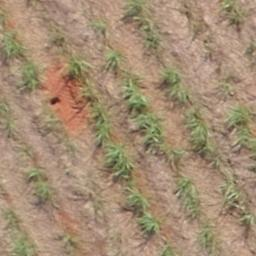
\includegraphics[width=\linewidth]{figures/tile_rgb.png}
\caption{RGB}
\end{subfigure}\hfill
\begin{subfigure}{0.31\columnwidth}
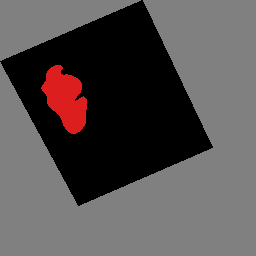
\includegraphics[width=\linewidth]{figures/tile_mask.png}
\caption{Máscara}
\end{subfigure}\hfill
\begin{subfigure}{0.31\columnwidth}
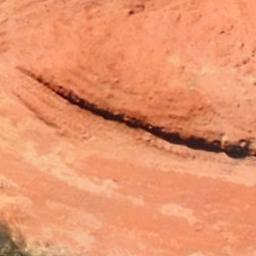
\includegraphics[width=\linewidth]{figures/tile_neg.png}
\caption{Negativo}
\end{subfigure}
\caption{Exemplos do dataset: (a) recorte RGB com formigueiro; (b) máscara correspondente (vermelho: formigueiro; preto: fundo; cinza: área ignorada); (c) recorte negativo de solo avermelhado, visualmente semelhante a um formigueiro.}
\label{fig:dataset}
\end{figure}

\paragraph{Pré-processamento das máscaras.} As máscaras RGB foram convertidas para três classes:

\begin{itemize}
    \item fundo: classe 0;
    \item formigueiro: classe 1;
    \item ignorado: classe 255.
\end{itemize}

A classe 255 foi utilizada para regiões não anotadas ou que não deveriam contribuir para o cálculo da função de perda. Esse tratamento evita que o modelo aprenda padrões incorretos em áreas fora da região de interesse.
%Durante o desenvolvimento, foram identificados valores inconsistentes nas máscaras após algumas transformações. Para corrigir esse problema, os rótulos foram padronizados de modo que apenas os valores 0, 1 e 255 fossem mantidos. Essa etapa foi fundamental para evitar ruído no treinamento supervisionado.

\paragraph{Transformações e normalização.}
As imagens foram normalizadas com média e desvio padrão do ImageNet. Embora o modelo tenha sido treinado no domínio agrícola, essa normalização contribui para estabilizar a escala dos dados de entrada.
As transformações geométricas, como rotações e espelhamentos, foram aplicadas de forma sincronizada entre imagem e máscara. Essa decisão é crítica em segmentação semântica, pois qualquer desalinhamento entre imagem e rótulo compromete diretamente o aprendizado.

\paragraph{Tratamento do desbalanceamento no nível de dados.}
O treinamento usa os recortes de $256\times256$ já prontos (cada recorte é um pedaço da ortofoto). Duas medidas reduzem o desbalanceamento já na preparação dos dados:

\begin{itemize}
    \item \textbf{Descarte de recortes quase vazios:} recortes cuja máscara tem mais de 70\% de área não anotada (classe \textit{ignorar}, típica das bordas) são removidos do treino, pois quase não trazem sinal de aprendizado e desperdiçam processamento.
    \item \textbf{Duplicação de formigueiros:} para o modelo ver mais exemplos da classe de interesse sem precisar de novas imagens, os formigueiros já presentes em um recorte são copiados para outras posições do próprio recorte. Isso ocorre em 70\% dos recortes com formigueiro, gerando até duas cópias, cada uma girada ou espelhada aleatoriamente; como a cópia permanece no mesmo recorte, o contexto (cor do solo e iluminação) continua realista (Figura~\ref{fig:aug}).
\end{itemize}

O desbalanceamento que resta (a pequena fração de pixels de formigueiro em cada imagem) é tratado pela função de custo combinada, apresentada a seguir.

\begin{figure*}[t]
\centering
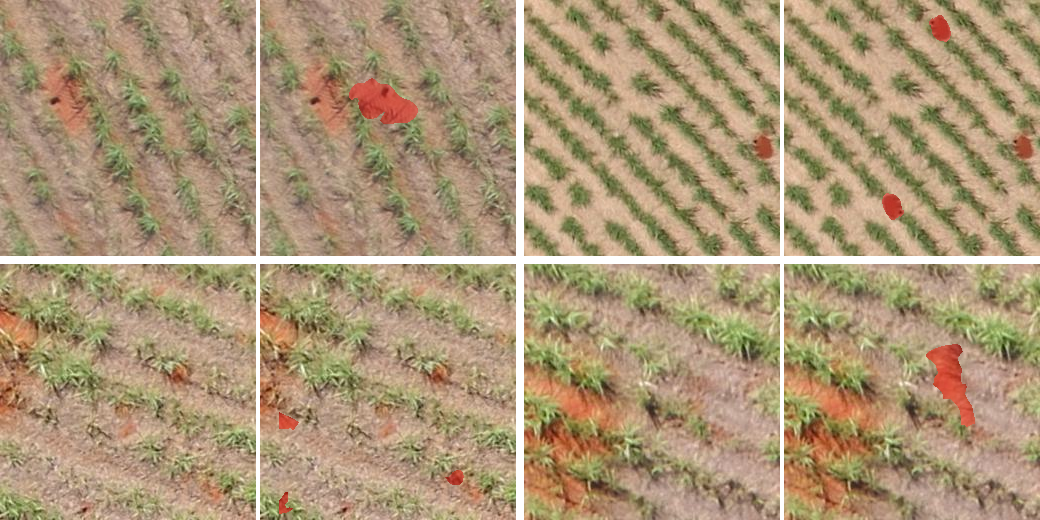
\includegraphics[width=0.9\textwidth]{figures/aug_anthill_duplicate.png}
\caption{Augmentação por duplicação de formigueiros (quatro exemplos). Em cada par, à esquerda o recorte original e à direita o recorte aumentado, com as novas cópias do formigueiro destacadas em vermelho; cada cópia é inserida em uma nova posição, com rotação e espelhamento aleatórios.}
\label{fig:aug}
\end{figure*}

\subsection{Arquitetura U-Net}

A arquitetura é uma U-Net totalmente convolucional, com um caminho de contração (encoder) e um de expansão (decoder) ligados por conexões de salto (\textit{skip connections}). A entrada é um recorte RGB de $3\times256\times256$. O encoder possui cinco estágios, com quatro reduções de resolução por \textit{max-pooling} $2\times2$; a profundidade de canais evolui em $64 \to 128 \to 256 \to 256 \to 1024$, enquanto a resolução cai de $256\times256$ até $16\times16$ (gargalo). Cada estágio aplica um bloco convolucional duplo: duas convoluções $3\times3$ (padding 1), cada uma seguida de Group Normalization (8 grupos) e ativação ReLU.

O decoder possui quatro estágios simétricos. Em cada um, uma convolução transposta $2\times2$ (passo 2) dobra a resolução, o resultado é concatenado com o mapa de características do estágio correspondente do encoder (\textit{skip connection}) e um bloco convolucional duplo refina a saída; a profundidade decresce $256 \to 256 \to 128 \to 64$. Uma convolução final $1\times1$ projeta para dois canais (fundo e formigueiro) na resolução original $256\times256$. A rede possui aproximadamente 19,7 milhões de parâmetros treináveis. A Tabela~\ref{tab:unet} detalha as camadas. As conexões de salto preservam detalhes finos de localização, importantes para segmentar regiões pequenas e de contorno irregular.

\begin{table}[H]
\centering
\caption{Detalhamento das camadas da U-Net (entrada RGB). Bloco duplo $=2\times$(Conv $3\times3$ pad 1 $+$ GroupNorm(8) $+$ ReLU); ConvT $=$ convolução transposta $2\times2$ (passo 2); concat $=$ concatenação com o \textit{skip} do encoder.}
\label{tab:unet}
\resizebox{\columnwidth}{!}{
\begin{tabular}{lll}
\toprule
\textbf{Estágio} & \textbf{Operação} & \textbf{Saída ($C\times H\times W$)} \\
\midrule
Entrada    & ---                              & $3\times256\times256$ \\
Enc1       & bloco duplo                      & $64\times256\times256$ \\
Enc2       & MaxPool $+$ bloco duplo          & $128\times128\times128$ \\
Enc3       & MaxPool $+$ bloco duplo          & $256\times64\times64$ \\
Enc4       & MaxPool $+$ bloco duplo          & $256\times32\times32$ \\
Gargalo    & MaxPool $+$ bloco duplo          & $1024\times16\times16$ \\
Dec1       & ConvT $+$ concat(Enc4) $+$ bloco & $256\times32\times32$ \\
Dec2       & ConvT $+$ concat(Enc3) $+$ bloco & $256\times64\times64$ \\
Dec3       & ConvT $+$ concat(Enc2) $+$ bloco & $128\times128\times128$ \\
Dec4       & ConvT $+$ concat(Enc1) $+$ bloco & $64\times256\times256$ \\
Saída      & Conv $1\times1$                  & $2\times256\times256$ \\
\bottomrule
\end{tabular}}
\end{table}

Além da normalização da entrada (média e desvio do ImageNet), descrita na preparação dos dados, a rede aplica normalização após cada convolução. Inicialmente utilizou-se Batch Normalization que, em conjunto com o upsampling aprendido por convolução transposta (ConvTranspose2d) no decoder, estabilizou o treinamento e foi decisiva para a evolução das métricas. Entretanto, devido à limitação de memória da GPU (6\,GB), o treinamento emprega lotes pequenos (\textit{batch size} = 2), regime no qual as estatísticas por lote do Batch Normalization tornam-se instáveis. Por esse motivo, o Batch Normalization foi substituído por Group Normalization (8 grupos), que normaliza grupos de canais de forma independente do tamanho do lote, preservando a estabilidade do treino. Como salvaguarda adicional contra explosão de gradientes, aplica-se recorte de gradiente (norma máxima 1,0).

Durante a inferência, a probabilidade da classe formigueiro é comparada a um limiar de confiança para gerar a máscara binária final.

\subsection{Função de custo e otimização}

Foram avaliadas diferentes estratégias de função de custo ao longo dos experimentos. A configuração baseline utilizou exclusivamente Cross-Entropy, servindo como referência para avaliar o impacto incremental das demais estratégias. Em seguida, foram aplicadas combinações com Tversky Loss \cite{salehi2017}, Focal Loss \cite{lin2017} e Lovász Loss \cite{berman2018} para lidar melhor com o desbalanceamento de classes e aproximar o treinamento da métrica de IoU.

A Tversky Loss é definida por:

\begin{equation}
\mathcal{L}_{T} = 1 - \frac{TP}{TP + \alpha FP + \beta FN},
\label{eq:tversky}
\end{equation}
em que $TP$, $FP$ e $FN$ representam verdadeiros positivos, falsos positivos e falsos negativos, respectivamente. Valores maiores de $\beta$ penalizam mais os falsos negativos, favorecendo maior Recall.

A Focal Loss reduz a contribuição de exemplos fáceis e concentra o gradiente em pixels difíceis:

\begin{equation}
\mathcal{L}_{F} = - \sum_i (1 - p_{t,i})^\gamma \log(p_{t,i}).
\label{eq:focal}
\end{equation}

A Lovász Loss \cite{berman2018} otimiza diretamente uma relaxação contínua do índice de Jaccard (IoU). No caso binário, define-se por pixel a margem $m_i = z_{i,1} - z_{i,0}$ (diferença entre os logits de formigueiro e de fundo) e o erro $e_i = 1 - m_i s_i$, com $s_i \in \{-1, +1\}$ indicando a classe verdadeira. Ordenando os erros de forma decrescente, a perda é

\begin{equation}
\mathcal{L}_{Lov} = \sum_i \max(0,\, e_{(i)})\, g_i,
\label{eq:lovasz}
\end{equation}
em que $e_{(i)}$ são os erros ordenados e $g$ é o gradiente da extensão de Lovász da perda de Jaccard, o que torna o IoU diferenciável.

A configuração final do modelo combina as três perdas:

\begin{equation}
\mathcal{L} = 0{,}5\,\mathcal{L}_{T} + 0{,}2\,\mathcal{L}_{F} + 0{,}3\,\mathcal{L}_{Lov}.
\label{eq:combined}
\end{equation}
Adotaram-se $\alpha = 0{,}3$ e $\beta = 0{,}7$ na Tversky (favorecendo o Recall), $\gamma = 2{,}0$ na Focal e peso de classe $6{,}0$ para formigueiro (e $1{,}0$ para fundo) na componente Focal; os pixels não anotados (rótulo 255) são ignorados em todas as componentes.

O otimizador utilizado foi Adam \cite{kingma2015}, com taxa de aprendizado inicial de $1 \times 10^{-3}$. Também foi utilizado controle de gradiente para evitar instabilidades durante o treinamento.

\subsection{Inferência e métricas de avaliação}

Na etapa de inferência, a máscara final é obtida aplicando um threshold sobre a probabilidade da classe formigueiro. Nos experimentos finais, o threshold de 0,40 foi utilizado para aumentar o Recall. Esse threshold influencia diretamente o trade-off entre Recall e Precision. Thresholds mais altos reduzem falsos positivos, porém aumentam falsos negativos. Thresholds menores aumentam a capacidade de identificação, mas ampliam a quantidade de regiões incorretamente classificadas.

Para avaliação, foram usadas Precision, Recall e F1-Score, que medem a capacidade do modelo de identificar corretamente a presença de formigueiros na imagem (Equação~\ref{eq:f1}), e IoU e Dice, que avaliam a qualidade espacial da segmentação pixel a pixel (Equação~\ref{eq:iou}). Nesse contexto, um modelo pode apresentar Recall elevado, indicando boa capacidade de detecção, mas IoU moderado, refletindo limitações na precisão geométrica das máscaras preditas.

\begin{equation}
F1 = 2 \cdot \frac{Precision \cdot Recall}{Precision + Recall}.
\label{eq:f1}
\end{equation}

\begin{equation}
IoU = \frac{TP}{TP + FP + FN}.
\label{eq:iou}
\end{equation}

Foram conduzidas catorze rodadas de treinamento (Run 01 a Run 14), das quais sete são detalhadas na Tabela~\ref{tab:comparacao}. Entre as rodadas, variaram-se quatro grupos de fatores:

\begin{itemize}
    \item \textbf{Função de custo:} de Cross-Entropy (\textit{baseline}) a combinações de Tversky, Focal e Lovász (Equação~\ref{eq:combined});
    \item \textbf{Augmentações:} espelhamento horizontal e vertical, rotação aleatória ($\pm15°$), variação fotométrica (brilho, contraste e saturação), deformação elástica ($\alpha=25$, $\sigma=4$) e augmentações da classe positiva (\textit{copy-paste} entre recortes nas rodadas intermediárias e duplicação intra-recorte na configuração final);
    \item \textbf{Limiar de confiança:} avaliado em diferentes valores, adotando-se $0{,}40$ na configuração final (Tabela~\ref{tab:threshold});
    \item \textbf{Filtragem de regiões conexas:} no pós-processamento, regiões muito pequenas ou muito grandes são descartadas; o tamanho mínimo passou de $100$ px nas primeiras rodadas para $5$ px na final, com máximo de $5.000$ px.
\end{itemize}

As métricas foram calculadas sobre o conjunto de validação (2.466 imagens), considerando tanto a detecção por imagem (Precision, Recall e F1-Score) quanto a segmentação pixel a pixel (IoU e Dice da classe formigueiro).

Os experimentos foram realizados em ambiente Linux Ubuntu, utilizando a biblioteca PyTorch para treinamento da rede neural. O treinamento foi executado em um computador com as seguintes especificações:

\begin{itemize}
    \item Processador Intel Core i5-10400F;
    \item 16 GB de memória RAM;
    \item GPU NVIDIA GeForce RTX 2060 com 6 GB de VRAM.
\end{itemize}



\section{Resultados e Discussão}

Os experimentos foram organizados em rodadas (\textit{runs}) numeradas, cada uma correspondendo a uma configuração de treinamento (arquitetura, função de custo, augmentações e pós-processamento), evoluídas de forma incremental a partir de um \textit{baseline} com Cross-Entropy. Esta seção destaca as rodadas que representam marcos dessa evolução, em especial a Run 05 (maior IoU) e a Run 14 (maior Recall e menor número de falsos negativos), esta última adotada como configuração final por priorizar a detecção em cenários de monitoramento. A Tabela~\ref{tab:comparacao} resume as configurações e os resultados das rodadas selecionadas.

\subsection{Calibração do limiar e desempenho final}

A Tabela~\ref{tab:threshold} apresenta o impacto de diferentes valores de threshold.

\begin{table}[H]
\centering
\caption{Impacto do threshold nas métricas de detecção.}
\label{tab:threshold}
\begin{tabular}{cccc}
\toprule
Threshold & Precision & Recall & F1-Score \\
\midrule
0,50 & 84,2\% & 85,2\% & 84,7\% \\
0,45 & 80,0\% & 87,7\% & 83,7\% \\
0,40 & 75,9\% & 91,7\% & 83,1\% \\
0,35 & 72,5\% & 94,1\% & 82,1\% \\
\bottomrule
\end{tabular}
\end{table}

O limiar é aplicado sobre a probabilidade da classe formigueiro: reduzi-lo classifica mais pixels como positivos, o que aumenta o Recall (menos falsos negativos), mas também eleva os falsos positivos e reduz a Precision. Esse efeito é monotônico na Tabela~\ref{tab:threshold}: ao baixar o limiar de 0,50 para 0,35, o Recall sobe de 85,2\% para 94,1\% ($+8{,}9$ pp), enquanto a Precision cai de 84,2\% para 72,5\% ($-11{,}7$ pp). O F1-Score, por ser a média harmônica das duas, atinge o máximo em 0,50 (84,7\%) e decresce à medida que o limiar diminui, pois o ganho de Recall não compensa a perda de Precision.

A escolha de 0,40 não corresponde, portanto, ao maior F1, mas a um compromisso deliberado em favor da detecção. No cenário de monitoramento, um falso negativo é operacionalmente mais custoso que um falso positivo: um formigueiro não detectado deixa de ser tratado, enquanto um falso alarme pode ser descartado em revisão manual. Com o limiar de 0,40, o Recall alcança 91,7\% (apenas 49 falsos negativos na Run~14), ao custo de cerca de 1,6 pp em F1 e 8 pp em Precision frente a 0,50. Limiares ainda menores, como 0,35, elevam o Recall a 94,1\%, mas a Precision de 72,5\% gera um volume de falsos alarmes que torna 0,40 um equilíbrio mais adequado. A Figura~\ref{fig:threshold-vis} ilustra o efeito do limiar sobre uma mesma predição.

\begin{figure}[H]
\centering
\begin{subfigure}{0.31\columnwidth}
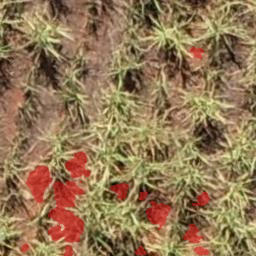
\includegraphics[width=\linewidth]{figures/thr_050.png}
\caption{$t=0{,}50$}
\end{subfigure}\hfill
\begin{subfigure}{0.31\columnwidth}
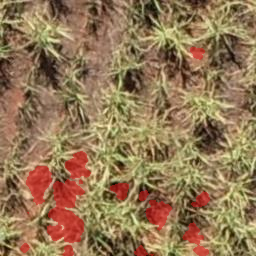
\includegraphics[width=\linewidth]{figures/thr_040.png}
\caption{$t=0{,}40$}
\end{subfigure}\hfill
\begin{subfigure}{0.31\columnwidth}
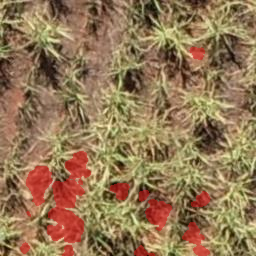
\includegraphics[width=\linewidth]{figures/thr_035.png}
\caption{$t=0{,}35$}
\end{subfigure}
\caption{Efeito do limiar de confiança $t$ sobre a mesma predição (região predita em vermelho). Limiares menores ampliam a área detectada (maior Recall), ao custo de mais falsos positivos.}
\label{fig:threshold-vis}
\end{figure}

A Run 14 é a configuração final do trabalho (linha correspondente na Tabela~\ref{tab:comparacao}): combina a loss Tversky+Focal+Lovász, GroupNorm, duplicação intra-recorte e limiar de 0,40, e foi escolhida por maximizar a detecção: maior Recall e menor número de falsos negativos. A Tabela~\ref{tab:run14det} apresenta seus resultados de detecção por imagem.

\begin{table}[H]
\centering
\caption{Resultados de detecção por imagem na Run 14.}
\label{tab:run14det}
\begin{tabular}{lr}
\toprule
\textbf{Métrica} & \textbf{Valor} \\
\midrule
TP & 544 \\
FP & 173 \\
FN & 49 \\
TN & 1.700 \\
Precision & 75,9\% \\
Recall & 91,7\% \\
F1-Score & 83,1\% \\
\bottomrule
\end{tabular}
\end{table}

A Tabela~\ref{tab:run14seg} apresenta os resultados pixel a pixel. Observa-se que a classe fundo obteve desempenho muito superior à classe formigueiro, reflexo direto do desbalanceamento dos dados.

\begin{table}[H]
\centering
\caption{Resultados de segmentação pixel a pixel na Run 14.}
\label{tab:run14seg}
\begin{tabular}{lr}
\toprule
\textbf{Métrica} & \textbf{Valor} \\
\midrule
Pixel Accuracy & 98,7\% \\
IoU fundo & 98,7\% \\
IoU formigueiro & 33,8\% \\
Dice formigueiro & 50,5\% \\
mIoU global & 66,3\% \\
Mean Dice global & 74,9\% \\
\bottomrule
\end{tabular}
\end{table}

Embora a acurácia global seja elevada, ela não deve ser interpretada isoladamente, pois a classe fundo domina a maior parte dos pixels. Por isso, o IoU da classe formigueiro é uma métrica mais representativa da qualidade da segmentação.

\subsection{Comparação entre rodadas}

A Tabela~\ref{tab:comparacao} resume as rodadas selecionadas como marcos da evolução, indicando a configuração de cada uma (arquitetura, função de custo e augmentações) e suas métricas. A seleção privilegia configurações representativas: a Run 03 (\textit{baseline} com Focal), a Run 05 (maior IoU), a Run 10 (melhor F1 equilibrado), as Runs 06, 08 e 11 (tentativas de melhoria que não superaram os marcos anteriores) e a Run 14 (maior Recall, configuração final).

\begin{table}[H]
\centering
\caption{Comparação entre configurações selecionadas.}
\label{tab:comparacao}
\resizebox{\columnwidth}{!}{
    \begin{tabular}{llrrrrr}
\toprule
\textbf{Run} & \textbf{Configuração} & \textbf{FP} & \textbf{FN} & \textbf{Precision} & \textbf{Recall} & \textbf{IoU form.} \\
\midrule
03 & U-Net base; Focal & 433 & 133 & 51,5\% & 77,6\% & 23,9\% \\
05 & + norm. + ConvT2d; Tversky+CE & 87 & 98 & 85,1\% & 83,5\% & \textbf{35,2\%} \\
06 & + oversampling 3:1 & 79 & 112 & \textbf{85,9\%} & 81,1\% & 34,3\% \\
08 & + copy-paste; elástica; rot90 & 44 & 187 & 90,2\% & 68,5\% & 34,2\% \\
10 & + Focal; copy-paste leve & 105 & 88 & 82,8\% & 85,2\% & 30,3\% \\
11 & + Lovász; filtro de tile & 60 & 171 & 87,6\% & 71,2\% & 28,5\% \\
14 & GroupNorm; + Lovász; duplic. intra-tile; limiar 0,40 & 173 & \textbf{49} & 75,9\% & \textbf{91,7\%} & 33,8\% \\
\bottomrule
\end{tabular}
}
\end{table}

Os resultados mostram um trade-off entre segmentação precisa e maior capacidade de detecção. Configurações mais conservadoras reduzem falsos positivos e podem melhorar o IoU, mas deixam de detectar parte dos formigueiros. Por outro lado, reduzir o threshold aumenta o Recall, mas também amplia falsos positivos em regiões visualmente semelhantes.

Para evidenciar a evolução incremental, a Tabela~\ref{tab:ablation} reúne as rodadas que marcaram cada etapa. Como cada rodada alterou mais de um fator simultaneamente, os ganhos não podem ser atribuídos isoladamente a um único componente; ainda assim, a progressão evidencia o efeito agregado das melhorias. O \textit{baseline} com Cross-Entropy não é incluído por ter colapsado para a classe de fundo, sem métricas úteis.

\begin{table}[H]
\centering
\caption{Evolução incremental ao longo das rodadas que marcaram cada etapa.}
\label{tab:ablation}
\resizebox{\columnwidth}{!}{
\begin{tabular}{llcc}
\toprule
Run & Principal mudança & Recall & IoU form. \\
\midrule
03 & U-Net base + Focal & 77,6\% & 23,9\% \\
05 & + normalização e ConvTranspose2d; Tversky+CE & 83,5\% & 35,2\% \\
10 & + Focal e augmentação (copy-paste, elástica) & 85,2\% & 30,3\% \\
14 & + Lovász, GroupNorm, duplicação intra-recorte, limiar 0,40 & \textbf{91,7\%} & 33,8\% \\
\bottomrule
\end{tabular}
}
\end{table}

Embora a Run 05 apresente o maior IoU (35,2\%), a configuração final (Run 14) foi escolhida por priorizar a detecção: seu Recall de 91,7\% supera em 8,2 pp o da Run 05, com apenas 49 falsos negativos (ante 98). O IoU ligeiramente menor (33,8\%) é um custo aceitável no monitoramento, em que deixar de detectar um formigueiro é mais grave que delimitá-lo com precisão imperfeita.

Vale destacar, contudo, que o maior ganho incremental observado (a passagem ao patamar de IoU em torno de 35\%) coincidiu com a estabilização da arquitetura, quando foram introduzidos a normalização nas convoluções e o upsampling aprendido (ConvTranspose2d). Como, nessa transição, a função de custo e a arquitetura foram alteradas de forma próxima, seus efeitos não podem ser plenamente isolados neste estudo, que utilizou uma única arquitetura. Mantida fixa a arquitetura nas etapas seguintes, as variações de desempenho passaram a ser governadas pelas estratégias de preparação de dados, escolha das funções de custo e calibração do limiar.

\subsection{Análise Qualitativa}

O modelo tem bom desempenho na maioria dos casos: formigueiros de tamanho médio a grande, isolados e com bom contraste em relação ao solo são detectados com alta confiança e máscaras bem delimitadas, o que se reflete no Recall de 91,7\%. O desempenho é mais consistente em solo escuro e uniforme, no qual a coloração do formigueiro se destaca do fundo. A Figura~\ref{fig:qual} apresenta exemplos de acerto, falso negativo e falso positivo.

\begin{figure*}[t]
\centering
\begin{subfigure}{0.8\textwidth}
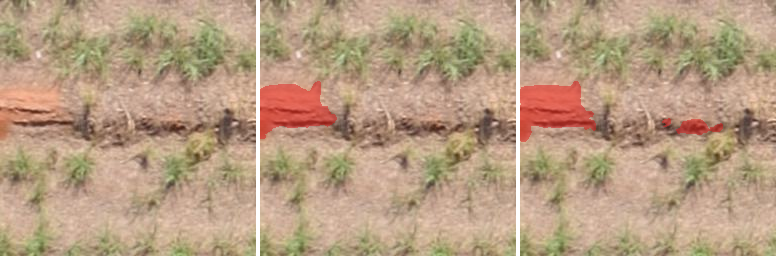
\includegraphics[width=\linewidth]{figures/qual_success.png}
\caption{Acerto}
\end{subfigure}

\begin{subfigure}{0.8\textwidth}
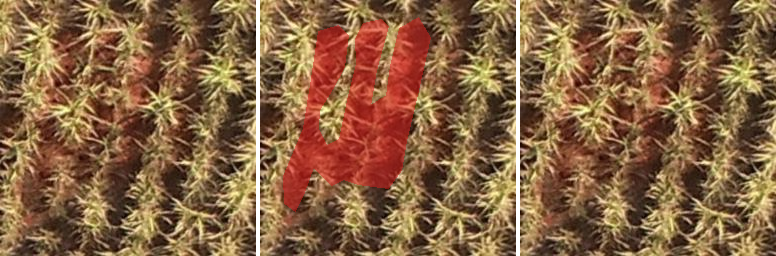
\includegraphics[width=\linewidth]{figures/qual_fn.png}
\caption{Falso negativo}
\end{subfigure}

\begin{subfigure}{0.8\textwidth}
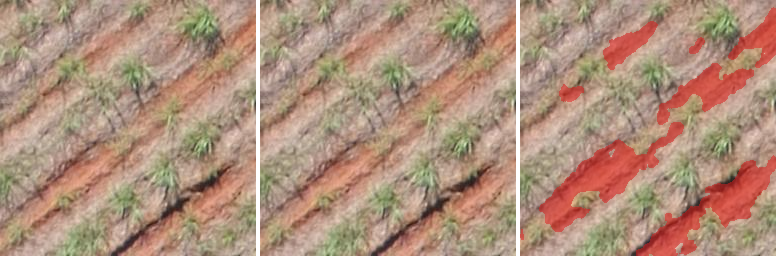
\includegraphics[width=\linewidth]{figures/qual_fp.png}
\caption{Falso positivo}
\end{subfigure}
\caption{Casos qualitativos na validação. Em cada linha, da esquerda para a direita: imagem RGB, ground-truth e predição da Run~14 (região em vermelho). (a) acerto; (b) falso negativo (formigueiro não detectado); (c) falso positivo em solo avermelhado.}
\label{fig:qual}
\end{figure*}

Os falsos negativos ocorreram principalmente em três situações: formigueiros muito pequenos, regiões com textura semelhante ao solo e imagens com grande quantidade de área ignorada. Esses casos reduzem a confiança do modelo e dificultam a separação entre alvo e fundo.

Os falsos positivos foram associados principalmente a solo avermelhado, marcas de pneus, linhas de cultivo e sombras. Esses padrões apresentam textura e coloração semelhantes aos formigueiros, levando o modelo a classificar incorretamente algumas regiões como positivas.

Essa análise indica que novas anotações devem priorizar exatamente esses casos difíceis. A inclusão de mais exemplos de solo avermelhado sem formigueiro e de formigueiros em contextos variados tende a melhorar a capacidade de generalização do modelo.

\section{Conclusão}

Este trabalho apresentou uma pipeline de segmentação semântica para detecção automática de formigueiros em ortofotos aéreas, baseada em U-Net e estruturada para lidar com forte desbalanceamento de classes. Os experimentos sustentam a hipótese de que melhorias sistemáticas na preparação de dados e no tratamento do desbalanceamento produzem ganhos substanciais na detecção e na segmentação da classe minoritária, partindo de um baseline de Cross-Entropy que tendia a colapsar para a classe de fundo. Ressalta-se, contudo, que o maior salto de desempenho coincidiu com a estabilização da arquitetura (introdução de normalização nas convoluções e de upsampling aprendido); como o estudo utilizou uma única arquitetura, os efeitos de dados e de arquitetura não puderam ser plenamente isolados, o que se registra como limitação e direção para trabalhos futuros.

Os resultados demonstraram que o modelo é capaz de detectar a maior parte dos formigueiros presentes no conjunto de validação, alcançando Recall de 91,7\% e F1-Score de 83,1\%. Entretanto, a qualidade da segmentação pixel a pixel ainda é limitada pela baixa representatividade da classe formigueiro e pela semelhança visual com regiões de solo exposto.

A análise experimental mostrou que a acurácia global não é suficiente para avaliar o problema, pois o fundo domina a maior parte dos pixels. Métricas específicas da classe de interesse, como IoU e Dice do formigueiro, são mais adequadas para medir a qualidade real da segmentação.

O trabalho também apresenta limitações. A baixa quantidade de exemplos positivos rotulados restringe a capacidade de generalização do modelo. Além disso, por utilizar apenas a arquitetura U-Net, sem comparação com modelos mais recentes (como DeepLabV3+ ou arquiteturas baseadas em Transformers), os efeitos da preparação de dados e os da arquitetura não puderam ser plenamente isolados; isolá-los exigiria reaplicar a mesma pipeline de dados a arquiteturas distintas. Por fim, não foram realizados testes em conjuntos externos ou em cenários operacionais reais de monitoramento agrícola.

Como trabalhos futuros, recomenda-se ampliar o conjunto de dados com novos exemplos positivos, incluir casos difíceis de falsos positivos e falsos negativos, testar backbones pré-treinados, avaliar estratégias de anotação ativa e explorar métodos de segmentação de instâncias para estimar individualmente cada formigueiro detectado.

\bibliographystyle{plain}
\begin{thebibliography}{99}

\bibitem{long2015}
Long, J.; Shelhamer, E.; Darrell, T.
Fully convolutional networks for semantic segmentation.
In: \textit{IEEE Conference on Computer Vision and Pattern Recognition}, 2015.

\bibitem{ronneberger2015}
Ronneberger, O.; Fischer, P.; Brox, T.
U-Net: Convolutional networks for biomedical image segmentation.
In: \textit{Medical Image Computing and Computer-Assisted Intervention}, 2015.

\bibitem{lin2017}
Lin, T.-Y. et al.
Focal loss for dense object detection.
In: \textit{IEEE International Conference on Computer Vision}, 2017.

\bibitem{milletari2016}
Milletari, F.; Navab, N.; Ahmadi, S.-A.
V-Net: Fully convolutional neural networks for volumetric medical image segmentation.
In: \textit{International Conference on 3D Vision}, 2016.

\bibitem{salehi2017}
Salehi, S. S. M.; Erdogmus, D.; Gholipour, A.
Tversky loss function for image segmentation using 3D fully convolutional deep networks.
In: \textit{Machine Learning in Medical Imaging}, 2017.

\bibitem{berman2018}
Berman, M.; Triki, A. R.; Blaschko, M. B.
The Lovász-Softmax loss: A tractable surrogate for the optimization of the intersection-over-union measure in neural networks.
In: \textit{IEEE Conference on Computer Vision and Pattern Recognition}, 2018.

\bibitem{kingma2015}
Kingma, D. P.; Ba, J.
Adam: A method for stochastic optimization.
In: \textit{International Conference on Learning Representations}, 2015.

\bibitem{buslaev2020}
Buslaev, A. et al.
Albumentations: Fast and flexible image augmentations.
\textit{Information}, v. 11, n. 2, 2020.

\bibitem{kamilaris2018}
Kamilaris, A.; Prenafeta-Boldú, F. X.
Deep learning in agriculture: A survey.
\textit{Computers and Electronics in Agriculture}, v. 147, p. 70--90, 2018.

\bibitem{mohanty2016}
Mohanty, S. P.; Hughes, D. P.; Salathé, M.
Using deep learning for image-based plant disease detection.
\textit{Frontiers in Plant Science}, v. 7, art. 1419, 2016.

\bibitem{milioto2018}
Milioto, A.; Lottes, P.; Stachniss, C.
Real-time semantic segmentation of crop and weed for precision agriculture robots leveraging background knowledge in CNNs.
In: \textit{IEEE International Conference on Robotics and Automation (ICRA)}, 2018.

\bibitem{sa2018}
Sa, I. et al.
WeedMap: A large-scale semantic weed mapping framework using aerial multispectral imaging and deep neural network for precision farming.
\textit{Remote Sensing}, v. 10, n. 9, art. 1423, 2018.

\bibitem{dellalucia2014}
Della Lucia, T. M. C.; Gandra, L. C.; Guedes, R. N. C.
Managing leaf-cutting ants: peculiarities, trends and challenges.
\textit{Pest Management Science}, v. 70, n. 1, p. 14--23, 2014.

\bibitem{tsouros2019}
Tsouros, D. C.; Bibi, S.; Sarigiannidis, P. G.
A review on UAV-based applications for precision agriculture.
\textit{Information}, v. 10, n. 11, art. 349, 2019.

\bibitem{dossantos2022}
dos Santos, A. et al.
Remote detection and measurement of leaf-cutting ant nests using deep learning and an unmanned aerial vehicle.
\textit{Computers and Electronics in Agriculture}, v. 198, art. 107071, 2022.

\bibitem{santos2019}
Santos, I. C. L. et al.
Remote sensing to detect nests of the leaf-cutting ant Atta sexdens (Hymenoptera: Formicidae) in teak plantations.
\textit{Remote Sensing}, v. 11, n. 14, art. 1641, 2019.

\bibitem{chatgpt}
OpenAI.
ChatGPT.
Disponível em: \url{https://chat.openai.com/}.

\end{thebibliography}

\end{document}